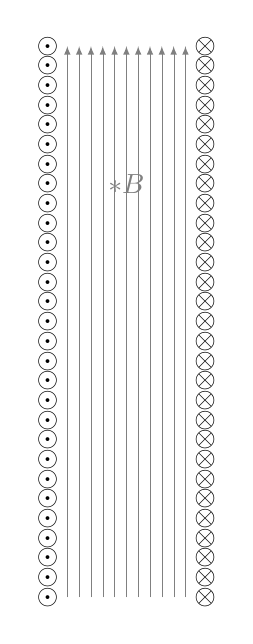
\begin{tikzpicture}[scale=1]
    \foreach \x in {-3.5,-3.25,...,3.5}
    {
        \node at (-1,\x) {$\odot$};
        \node at (+1,\x) {$\otimes$};
    }
    % \draw (0,0) circle (2.37);
    % \draw (0,0) circle (3.38);

    \foreach \x in {-0.75,-0.6,...,0.76}
    {
        \draw[-latex,ultra thin,gray] (\x,-3.5)--(\x,3.5);
    }

    \node[gray,above] at (0,1.5) {$\vb*{B}$};
\end{tikzpicture}
